\documentclass[border=6pt]{standalone}
\usepackage{tikz}
\usepackage{amsmath,amssymb}
\usetikzlibrary{arrows.meta, positioning, calc, fit}

\begin{document}
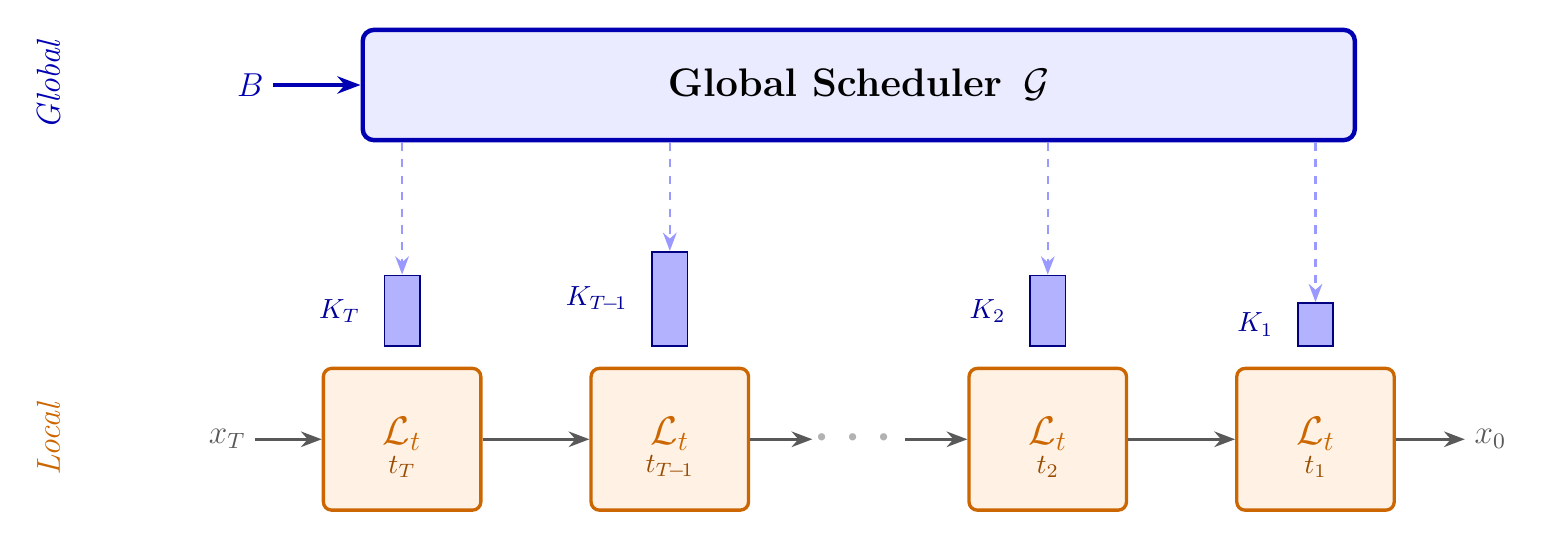
\begin{tikzpicture}[
    >=Stealth,
    localbox/.style={
      draw=orange!80!black, fill=orange!10, rounded corners=3pt,
      minimum width=2.0cm, minimum height=1.8cm, line width=1.2pt,
    },
    budgetbar/.style={
      draw=blue!50!black, fill=blue!30, minimum width=0.45cm,
      line width=0.6pt
    },
    every node/.style={font=\normalsize},
    dashed arrow/.style={->, dashed, blue!40, line width=0.8pt},
    flow arrow/.style={->, gray!70!black, line width=1pt},
  ]

  %% ---- layout: uniform arrow gaps ----
  %% box width = 2.0cm, so radius = 1.0cm
  %% edge-to-edge gap between adjacent boxes = 1.4cm
  %% dots occupy ~0.8cm, with 1.0cm arrow on each side
  \def\boxy{0}

  % Box centers (explicit for uniform gaps)
  \node[localbox] (LT)   at (0, \boxy)    {};
  \node[localbox] (LT1)  at (3.4, \boxy)  {};
  \node[localbox] (L2)   at (8.2, \boxy)  {};
  \node[localbox] (L1)   at (11.6, \boxy) {};

  % L_t labels inside boxes
  \node[font=\Large, orange!80!black] at ([yshift=2pt]LT.center)
    {$\mathcal{L}_t$};
  \node[font=\Large, orange!80!black] at ([yshift=2pt]LT1.center)
    {$\mathcal{L}_t$};
  \node[font=\Large, orange!80!black] at ([yshift=2pt]L2.center)
    {$\mathcal{L}_t$};
  \node[font=\Large, orange!80!black] at ([yshift=2pt]L1.center)
    {$\mathcal{L}_t$};

  % t_i subscripts
  \node[font=\normalsize, orange!60!black] at ([yshift=-10pt]LT.center)
    {$t_T$};
  \node[font=\normalsize, orange!60!black] at ([yshift=-10pt]LT1.center)
    {$t_{T\!-\!1}$};
  \node[font=\normalsize, orange!60!black] at ([yshift=-10pt]L2.center)
    {$t_2$};
  \node[font=\normalsize, orange!60!black] at ([yshift=-10pt]L1.center)
    {$t_1$};

  %% ---- cdots (centered between LT1 and L2) ----
  \node[font=\Huge, gray!60, inner sep=0pt] (dots)
    at ($(LT1.east)!0.5!(L2.west)$) {$\cdots$};

  %% ---- budget bars above local boxes ----
  \def\bargap{0.25}
  \node[budgetbar, minimum height=0.9cm, anchor=south]
    (barT)  at ([yshift=\bargap cm]LT.north)  {};
  \node[budgetbar, minimum height=1.2cm, anchor=south]
    (barT1) at ([yshift=\bargap cm]LT1.north) {};
  \node[budgetbar, minimum height=0.9cm, anchor=south]
    (bar2)  at ([yshift=\bargap cm]L2.north)   {};
  \node[budgetbar, minimum height=0.55cm, anchor=south]
    (bar1)  at ([yshift=\bargap cm]L1.north)   {};

  %% ---- K labels to the left of each bar ----
  \node[font=\normalsize, blue!60!black, anchor=east]
    at ([xshift=-5pt]barT.west)  {$K_T$};
  \node[font=\normalsize, blue!60!black, anchor=east]
    at ([xshift=-5pt]barT1.west) {$K_{T\!-\!1}$};
  \node[font=\normalsize, blue!60!black, anchor=east]
    at ([xshift=-5pt]bar2.west)  {$K_2$};
  \node[font=\normalsize, blue!60!black, anchor=east]
    at ([xshift=-5pt]bar1.west)  {$K_1$};

  %% ---- global scheduler box ----
  \node[draw=blue!70!black, fill=blue!8, rounded corners=4pt,
        minimum width=12.6cm, minimum height=1.4cm, line width=1.6pt,
        font=\Large, anchor=south]
    (G) at ($(LT.north)!0.5!(L1.north) + (0, 2.85)$)
    {\textbf{Global Scheduler}\;\;$\mathcal{G}$};

  %% ---- B arrow into global box ----
  \node[font=\large, blue!70!black] (B) at ([xshift=-1.4cm]G.west) {$B$};
  \draw[flow arrow, blue!70!black, line width=1.2pt]
    (B.east) -- (G.west);

  %% ---- dashed arrows: global scheduler -> bar tops ----
  \draw[dashed arrow] (G.south -| barT)  -- (barT.north);
  \draw[dashed arrow] (G.south -| barT1) -- (barT1.north);
  \draw[dashed arrow] (G.south -| bar2)  -- (bar2.north);
  \draw[dashed arrow] (G.south -| bar1)  -- (bar1.north);

  %% ---- horizontal flow arrows (uniform length, no overlap) ----
  % x_T -> LT
  \node[font=\large, gray!70!black] (xT) at ([xshift=-1.2cm]LT.west) {$x_T$};
  \draw[flow arrow] (xT.east) -- (LT.west);

  % LT -> LT1  (gap = 1.4cm)
  \draw[flow arrow] (LT.east) -- (LT1.west);

  % LT1 -> short arrow -> dots -> short arrow -> L2
  \draw[flow arrow] (LT1.east) -- (dots.west);
  \draw[flow arrow] (dots.east) -- (L2.west);

  % L2 -> L1  (gap = 1.4cm)
  \draw[flow arrow] (L2.east) -- (L1.west);

  % L1 -> x_0
  \node[font=\large, gray!70!black] (x0) at ([xshift=1.2cm]L1.east) {$x_0$};
  \draw[flow arrow] (L1.east) -- (x0.west);

  %% ---- side labels (far left, no overlap) ----
  \coordinate (sidelabel) at ([xshift=-3.2cm]LT.west);
  \node[font=\large\itshape, blue!70!black, rotate=90, anchor=south]
    at (sidelabel |- G.center) {Global};
  \node[font=\large\itshape, orange!80!black, rotate=90, anchor=south]
    at (sidelabel |- LT.center) {Local};

\end{tikzpicture}
\end{document}
